\section{Prérequis}
\subsection{Bases de l'informatique}
\[
  \mathtt{0b101010} = 1\times 2^5 + 0\times 2^4 + 1\times 2^3
  + 0\times 2^2 + 1\times 2^1 + 0\times 2^0 = 32 + 8 + 2 = 42.
\]

\begin{figure}[h!]
  \centering
  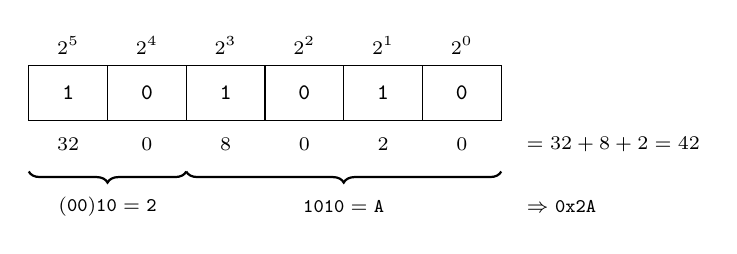
\begin{tikzpicture}[font=\footnotesize]
    \foreach \b [count=\i from 0] in {1,0,1,0,1,0} {
      \pgfmathtruncatemacro{\w}{5-\i}
      \pgfmathtruncatemacro{\val}{\b*(2^(5-\i))}
      \draw (\i,0) rectangle ++(1,0.7);
      \node at (\i+0.5,0.35) {\texttt{\b}};
      \node[font=\scriptsize] at (\i+0.5,0.95) {$2^{\w}$};
      \node[font=\scriptsize] at (\i+0.5,-0.3) {\val};
    }
    \node[anchor=west,font=\scriptsize] at (6.2,-0.3) {$=32+8+2=42$};
    \draw[decorate,decoration={brace,amplitude=4pt,mirror},thick]
      (0,-0.65) -- (2,-0.65);
    \draw[decorate,decoration={brace,amplitude=4pt,mirror},thick]
      (2,-0.65) -- (6,-0.65);
    \node[font=\scriptsize] at (1,-1.1) {$\mathtt{(00)10}=\mathtt{2}$};
    \node[font=\scriptsize] at (4,-1.1) {$\mathtt{1010}=\mathtt{A}$};
    \node[anchor=west,font=\scriptsize] at (6.2,-1.1) {$\Rightarrow \mathtt{0x2A}$};
  \end{tikzpicture}
\end{figure}

Hexadecimal uses the digits $0$ to $9$ and then $\mathtt{A}\,(=10)$ to
$\mathtt{F}\,(=15)$, so that
\[
  \mathtt{0x2A} = 2\times 16^1 + 10 = 32 + 10 = 42.
\]
\begin{notation}[Prefixes]
  \texttt{0b} marks une représentation binaire and \texttt{0x} celle
  hexadécimale. C uses these same prefixes.
\end{notation}

\subsubsection{Endianness (petit-boutien / grand-boutien)}
\begin{definition}[Grand-boutien (\textit{big-endian}) and petit-boutien (\textit{little-endian})]
  In \textbf{grand-boutien} order the octets are written classically with the
  most significant octet first. In \textbf{petit-boutien} order, often when the
  size of the words is known, the least significant octet comes first: if $m =
  o_1 o_2$ then
  \[
    m = o_1 + 256\, o_2 .
  \]
\end{definition}
\begin{figure}[h!]
  \centering
  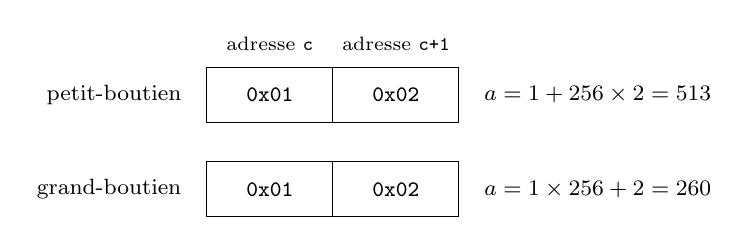
\begin{tikzpicture}[font=\footnotesize]
    % little endian
    \node[anchor=east] at (-0.2,1.35) {petit-boutien};
    \draw (0,1) rectangle ++(1.6,0.7); \node at (0.8,1.35) {\texttt{0x01}};
    \draw (1.6,1) rectangle ++(1.6,0.7); \node at (2.4,1.35) {\texttt{0x02}};
    \node[anchor=west] at (3.4,1.35)
      {$a = 1 + 256\times 2 = 513$};
    % big endian
    \node[anchor=east] at (-0.2,0.15) {grand-boutien};
    \draw (0,-0.2) rectangle ++(1.6,0.7); \node at (0.8,0.15) {\texttt{0x01}};
    \draw (1.6,-0.2) rectangle ++(1.6,0.7); \node at (2.4,0.15) {\texttt{0x02}};
    \node[anchor=west] at (3.4,0.15)
      {$a = 1\times 256 + 2 = 260$};
    % addresses
    \node[font=\scriptsize] at (0.8,2.0) {adresse \texttt{c}};
    \node[font=\scriptsize] at (2.4,2.0) {adresse \texttt{c+1}};
  \end{tikzpicture}
\end{figure}
\begin{remark}
  x86-64 is petit-boutien and is used hereinafter.
\end{remark}

\subsection{Complément à Deux}
Negative integers are represented in \textbf{complement à deux} (\textit{two's
complement}) on $k$ bits.\\

Mathematically, this allows the numbers to live in $\zee/2^{k}\zee$. The
operations $+$, $-$ and $\times$ then work regardless of whether the operands
are positive or negative. This does \emph{not} extend to comparisons and to
division.

\begin{definition}[Complement à Deux]
  The bit string $b_0 \ldots b_k$ represents
  \[
    -2^{k} b_{k} + \sum_{i<k} b_i 2^{i}.
  \]
  The most significant bit is a sign bit: $-1$ is written
  $\mathtt{0xFFFF}\ldots$, and the sign bit is used to invert the comparisons.
\end{definition}

\begin{figure}[h!]
  \centering
  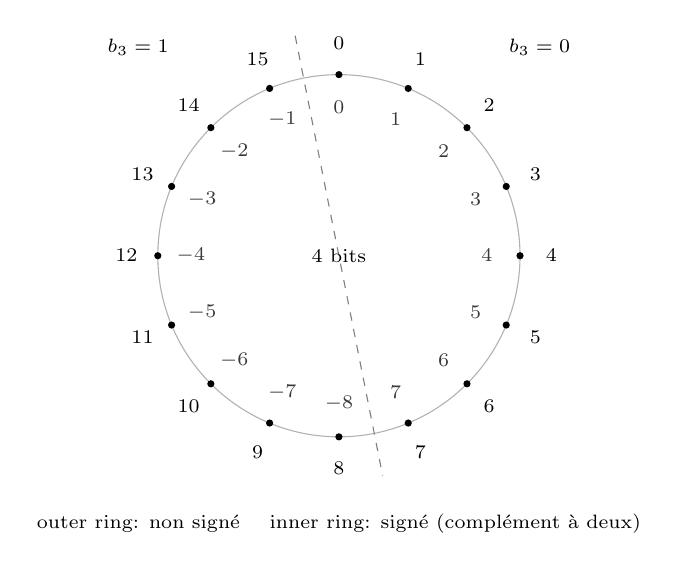
\begin{tikzpicture}[font=\scriptsize]
    \def\R{2.3}
    \draw[gray!60] (0,0) circle (\R);
    \draw[dashed,gray] (101.25:\R+0.55) -- (-78.75:\R+0.55);
    \foreach \u in {0,...,15} {
      \pgfmathsetmacro{\ang}{90 - \u*22.5}
      \pgfmathtruncatemacro{\s}{\u<8 ? \u : \u-16}
      \fill (\ang:\R) circle (1.3pt);
      \node at (\ang:\R+0.40) {\u};
      \node[gray!45!black] at (\ang:\R-0.42) {$\s$};
    }
    \node[font=\scriptsize,align=center] at (0,0) {4 bits};
    \node[font=\scriptsize] at (-2.55,\R+0.35) {$b_3=1$};
    \node[font=\scriptsize] at (2.55,\R+0.35) {$b_3=0$};
    \node[font=\scriptsize,anchor=north] at (0,-\R-0.85)
      {outer ring: non signé \quad inner ring: signé (complément à deux)};
  \end{tikzpicture}
\end{figure}

\begin{example}[Eight bits]
  $\mathtt{0x00}=0$, $\mathtt{0x7F}=127$, $\mathtt{0x80}=-128$,
  $\mathtt{0xFF}=-1$. The last follows from the formula: all bits set gives
  $-2^7 + (2^7-1) = -1$.
\end{example}

\subsection{Code ASCII}
ASCII is a table of characters on $7$ bits, i.e.\ the range $[0-127]$. It
covers the basic US characters and a set of ``control'' characters.
\begin{center}
  \includegraphics[width=0.75\textwidth]{ascii-table.pdf}
\end{center}

\subsection{Unités de Mémoire}
The definitions used in these notes for memory units are those of the C
standard, which are also those of the x86-64 architecture. The table below
gives the size of each unit and the number of values it can represent.
\begin{center}
  \begin{tabular}{lcc}
    \toprule
    & taille & \#~valeurs \\
    \midrule
    bit         & ---       & $2$ \\
    octet/byte  & 8 bits    & $256$ \\
    mot/word    & 2 octets  & $65\,536$ \\
    double      & 4 octets  & $\sim 4\cdot 10^{9}$ \\
    quad        & 8 octets  & $\sim 18\cdot 10^{18}$ \\
    \bottomrule
  \end{tabular}
  \hspace{1.2cm}
  \begin{tabular}{lcc}
    \toprule
    Type C & mini & courant \\
    \midrule
    \texttt{char}      & 8  & 8  \\
    \texttt{short}     & 16 & 16 \\
    \texttt{int}       & 16 & 32 \\
    \texttt{long}      & 32 & 64 \\
    \texttt{long long} & 64 & 64 \\
    \bottomrule
  \end{tabular}
\end{center}

\begin{remark}
  \textit{mot} désigne parfois le nombre de bits du processeurs (64 sur les
  processeurs modernes).
\end{remark}

The table on the right gives, for each C type, the width the standard
\emph{guarantees} and the width used in common implementations.

\subsection{Rappels de C}
C'est un langage de programmation qui est \textbf{proche de la machine}
(\textit{low-level}), \textbf{impératif}, avec \textbf{passage par valeur}
(\textit{pass-by-value}), \textbf{statiquement typé}, et l'indentation ne joue
aucun rôle (contrairement à Python).
